% !TEX encoding = UTF-8 Unicode

\Chapter{Apache Kafka}
Az Apache Kafka Scala és Java nyelven íródott, és a korábbi LinkedIn adatmérnökök alkotása. Már 2011-ben a technológiát erősen skálázható üzenetküldő rendszerként adták át amely nyílt forráskódú. Ma az Apache Kafka a Confluent Stream Platform része és napi események billióit kezeli. Az Apache Kafka számos megbízható társasággal körbeépítette magát a piacon.

A mai összetett rendszerekben szereplő adatokat és naplókat feldolgozni, újrafeldolgozni, elemezni és kezelni kell - gyakran valós időben. És ezért az Apache Kafka jelentős szerepet játszik az üzenet streaming környezetében. A Kafka kulcsfontosságú tervezési alapelveit az egyre növekvő igény alapján alakítják ki a nagy teljesítményű architektúrák, amelyek könnyen skálázhatóak, és lehetővé teszik az adatok tárolását, feldolgozását és újrafeldolgozását.

\Section{Kafka architektúra}
 \begin{figure}[ht]
	\centering
	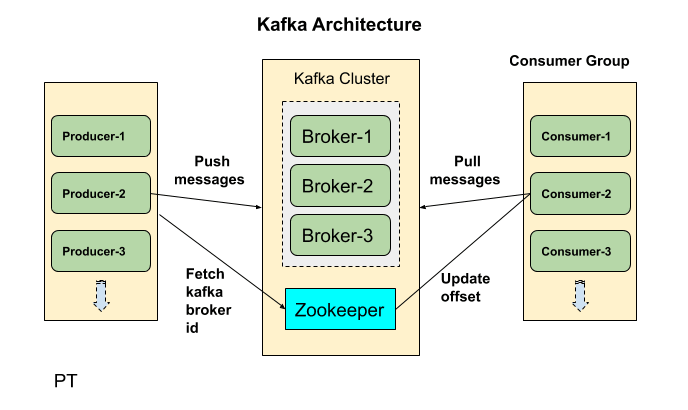
\epsfig{file=images/kafka-architecture.png,scale=0.45}
	\caption{Kafka architektúra} 
	\label{fig:kafka-architecture}
\end{figure}
Egy Kafka architektúra legalább egy Kafka szerverből (bróker) áll ami a konfigurációját kötelezően a Zookeeper nevű elosztott konfigurációs management rendszerben tárolja.  A Kafka borker-hez csatlakoznak a termelők és fogyasztók. A Kafka cluster-ben úgynevezett topic-ok találhatók. A termelők mindig egy dedikált topik-ra írnak, és a fogyasztók mindig egy dedikált topic-ról olvasnak, tehát a topic az a logikai egység, ami egy termelő-fogyasztó páros számára az üzeneteket tárolja és továbbítja.Mikor elindítunk egy Kafa példányt, akkor valójában egy kafka brokert indítunk el. Ha producer-ek mindig egy brokerhez csatlakoznak. A teljes konfiguráció zookeeper-ben van tárolva. A zookeeper tudja értesíteni a klienseket ha a konfiguráció változik, ezért hamar elterjed a hálózaton a változás. \Aref{fig:kafka-architecture} ábrán láthatjuk az architektúrát.\newline


\Section{Kafka működése}
Egy topic úgynevezett partíciókra van osztva. Minden üzenet csak egy partícióba kerül be. \Aref{fig:kafka-partitions} ábrán látható a partíció.
A producer-ek egy megadott topic-kra dobálják be az üzeneteket, amit onnan a consumer-ek kiolvasnak. Egy topic tetszőleges számú partícióból állhat. Egy partíció az a logikai egység, aminek rá kell férnie egy lemezre. A topic-kot úgy kell felskálázni, hogy egyre több partíciót adunk hozzá, amik különböző brokereken fognak létrejönni. Minden partíciónak lehet egy vagy több replikája, amik biztonsági másolatok. Mikor a producer beküld egy üzenetet egy partícióba, akkor fog committed üzenetnek minősülni, ha minden replikára is eljutott.
\begin{figure}[ht]
	\centering
	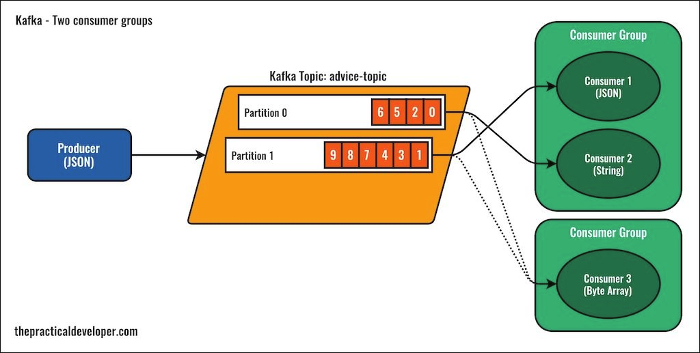
\epsfig{file=images/kafka-partitions.png,scale=0.45}
	\caption{Kafka partíciók} 
	\label{fig:kafka-partitions}
\end{figure}
Azt, hogy egy producer melyik partícióba dobja az üzenetet vagy a kulcs határozza meg, vagy round-robin módon mindig egy másikba teszi. Ha van kulcs, akkor az abból készült hash fogja meghatározni, hogy melyik partícióba kerüljön. Ugyan az a kulcs így mindig ugyan abba a partícióba fog kerülni. De a kulcs nem kötelező. A sorrend tartás csak egy partíción belül garantált, de ott nagyon. Ha nagyon kritikus bizonyos üzenetek sorrendje, akkor azokat egy partícióba kell rakni azonos kulcsot használva. Loggolásnál ez nem kritikus, egyrészt mert a logstash sorba rakja az üzeneteket, másrészt mikor elastichsearch-be szúrjuk, ott a dátum lesz az egyik attribútum, ami alapján már sorba lehet majd újra rendezni a logokat. Az meg amúgy sem kritikus, ha a log egy része enyhe csúszással kerül be az adatbázisba, lényeg, hogy végül helyes lesz a sorrend.

A comsumer-eket úgynevezett consumer-group-okba szervezzük az azonosítójuk szerint. Egy csoport mindig ugyan azon topic üzeneteit olvassa, de minden egyes consumer a csoporotban más és más partícióból. Minden partíció csak egy consumer-hez rendelhető hozzá egy csoporton belül. De ha nincs annyi consumer a csoportban mind ahány partíció, akkor egy consumer több partíciót is fog olvasni (ahogy ez a fenti ábrán is látszik, az alsó consumer két partíciót olvas. Viszont ha több consumer van mint partíció egy csoportban, akkor bizonyos consumer-ek mindig idle állapotban lesznek. Minden csoporton belül van egy vezető consumer, általában az aki először csatlakozott. Ő teríti a többieknek a cluster információkat.

A Kafka nem tudja értelmezni sem a kulcsot sem az üzenetet. Ez számára egy bájt tömb. Az, hogy egy objektumból hogy lesz bájt tömb kulcs és bájt tömb üzenet a producer-ben lévő serializátor dolga. A consumer-ben pedig a deserializázor dolga, hogy a bájt folyamból újra értelmes objektumot állítson elő.

Minden partíció új üzenete mindig a partíció végére íródik. A partíció elejétől számoljuk az üzenetek sorszámát, ezt hívjuk offset-nek. Mikor egy consumer kiolvas egy üzentet, attól az még ott marad a partícióba egészen addig, amíg len nem jár, alapértelmezetten ez egy nap. Tehát ez eltér a hagyományos sor kezeléstől. A Kafka nyilvántartja, hogy melyik consumer egy adott partícióban melyik offset-nél tartott. Ezt egy speciális topic-ban tartja nyilván: Ha újra is indul a világ, akkor is tudni fogják a consumer-ek hogy hol tartottak, és onnan folytatják.

\Section{Kafka és a logolás}

A docker alapú cloud világban egy tipikus architektúra a logok centralizált gyűjtésére, mikor egy logstash példány a producer és egy másik logstash példány a consumer. A konténer logokat a producer logstash kapja meg, aki a log sorok különböző paraméterei mentén a megfelelő Topic-ba tudja irányítani az üzeneteket. A consumer logstash pedig leszedi a Topic-rol az üzenetet és beírja Elasticsearch-be. \Aref{fig:kafka-elastic}

\begin{figure}[ht]
	\centering
	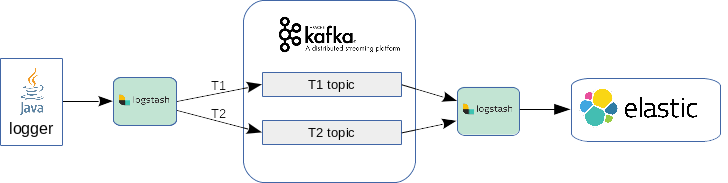
\epsfig{file=images/kafka-elastic.png,scale=0.45}
	\caption{Kafka és a Java} 
	\label{fig:kafka-elastic}
\end{figure}

A Kafka világban nagyon széles a választéka a producer-eknek és consumer-eknek, akik képesek közvetlenül Kafka-ba írni és onnan olvasni. A Java világban a megfelelő Kafka lib-ek segítségével írhatunk Java producer-eket és consumer-eket amik olyan Java programok, amik közvetlenül írják ill. olvassák a Kafka topic-ot. A másik lehetőség a producer-re, hogy a logger keretrendszerünk Kafka kliens appender-jét használjuk, ami a rendszer logokat képes kapásból Kafka-ba írni. Ha letöltjük a Kafka programot, akkor abban található parancssori producer és consumer is, ami képes tesztelés céljából közvetlen beírni és kiolvasni egy topic-ból, ami nagyon hasznos a tesztelés során.

\begin{figure}[ht]
	\centering
	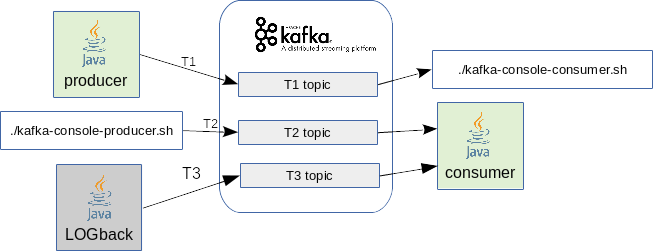
\epsfig{file=images/kafka-java.png,scale=0.45}
	\caption{Kafka logs} 
	\label{fig:kafka-java}
\end{figure}

     